
\begin{frame}{Types: \code{genus}}
  \centering
  
    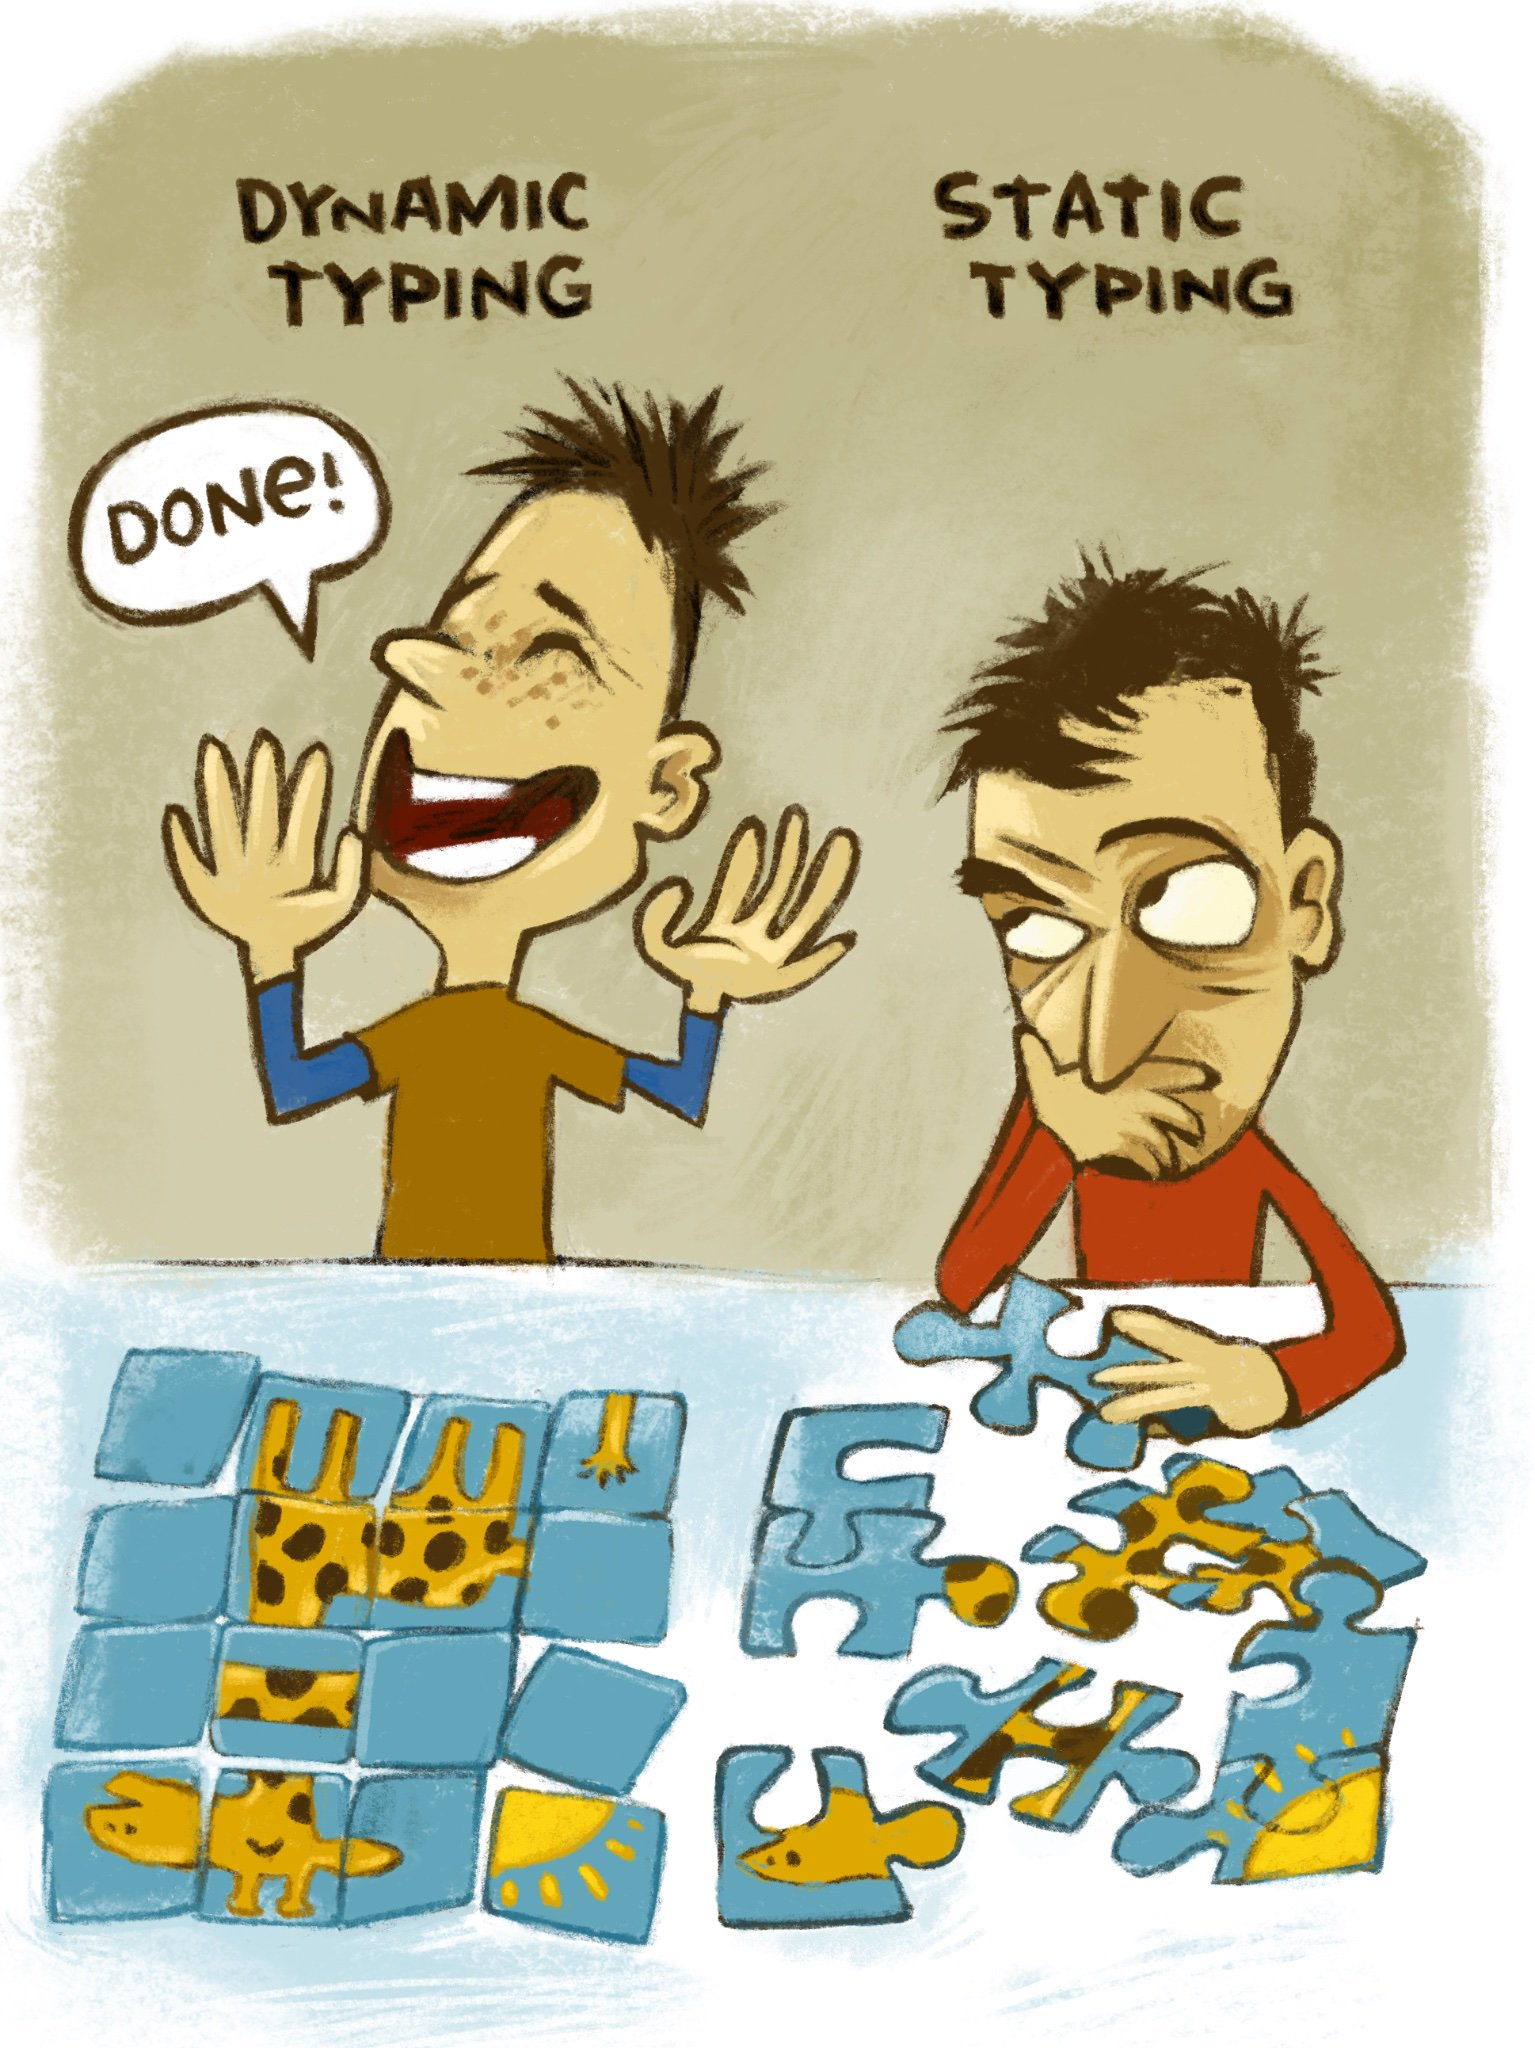
\includegraphics[height=8cm]{typing.png}
\end{frame}

\begin{frame}{Types}{What are Types?}
  \begin{itemize}
  \item Types as Sets
  \item Static
  \item Dynamic
  \end{itemize}
\end{frame}

\begin{frame}{SETS}{Simple Embedded Type System}

  \scalebox{1.0}{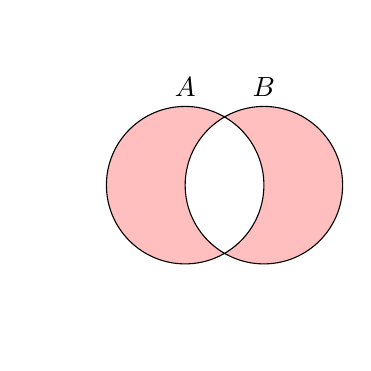
\begin{tikzpicture}[fill=pink]
% left hand
\scope
\clip (-2,-2) rectangle (2,2)
      (1,0) circle (1);
\fill (0,0) circle (1);
\endscope
% right hand
\scope
\clip (-2,-2) rectangle (2,2)
      (0,0) circle (1);
\fill (1,0) circle (1);
\endscope
% outline
\draw (0,0) circle (1) (0,1)  node [text=black,above] {$A$}
      (1,0) circle (1) (1,1)  node [text=black,above] {$B$};
\end{tikzpicture}
}

  \begin{itemize}
  \item   Extends type system of language (Scala, Python, Clojure)
  \item   Modeled on Common Lisp type system.
  \item   Supports intersection, union, complement.
  \item   Supports deterministic \Emph{membership check}.
  \item   Supports incomplete \Emph{subtype check}.
  \end{itemize}
\end{frame}

\begin{frame}{\code{SimpleTypeD} class quasi-ADT}
  \scalebox{0.8}{% Modeled after the following
% A simple Tree
% Author: Stefan Kottwitz
% https://www.packtpub.com/hardware-and-creative/latex-cookbook
\documentclass[border=10pt]{standalone}
\usepackage{tikz}
\begin{document}
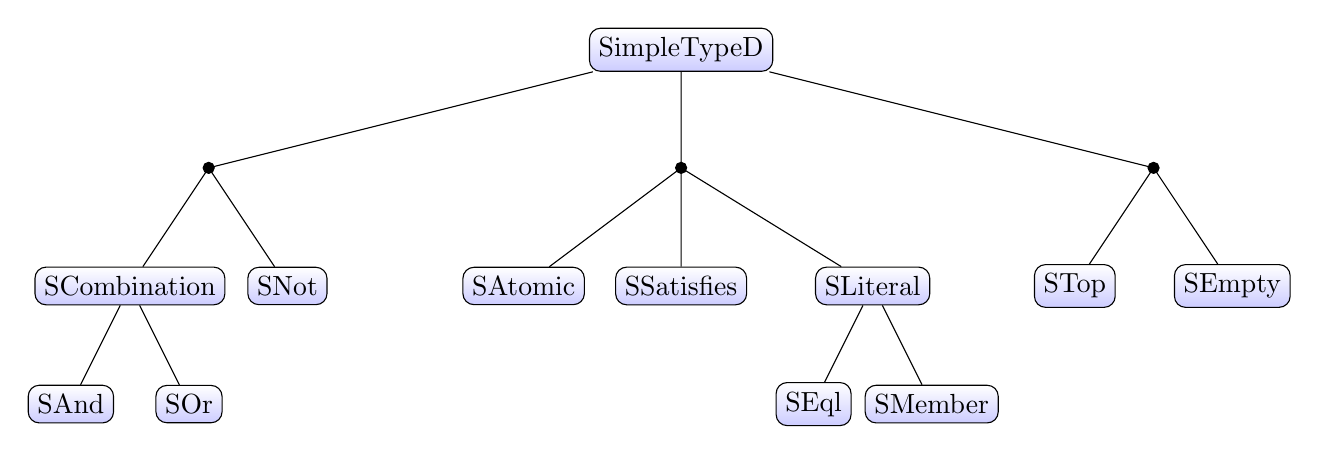
\begin{tikzpicture}[sibling distance=10em,
  every node/.style = {shape=rectangle, rounded corners,
    draw, align=center,
    top color=white, bottom color=blue!20}]]
    \tikzstyle{level 1}=[sibling distance=60mm]
    \tikzstyle{level 2}=[sibling distance=20mm]
    \tikzstyle{level 3}=[sibling distance=15mm]
  \node {SimpleTypeD}
    child { [fill] circle (2pt)
      child { node {SCombination} 
        child { node {SAnd} }
        child { node {SOr} } }
      child { node {SNot} } }
    child { [fill] circle (2pt)
      child { node {SAtomic} }
      child { node {SSatisfies} }
      child { node [right=-3mm] {SLiteral}
        child { node {SEql} }
        child { node {SMember} } } }
    child { [fill] circle (2pt)
      child { node {STop} }
      child { node {SEmpty} } } ;
\end{tikzpicture}
\end{document}
}

  \medskip

  Not an ADT for a \Emph{silly} reason.

  Scala does not support cross-file \code{sealed} classes.
\end{frame}


\begin{frame}{SimpleTypeD}{As quasi-Alebraic Data Type}

  \begin{columns}

    \begin{column}{0.4\textwidth}
  
      %% By Watchduck author "T. Piesk", "Tilman Piesk" or
      %% "Watchduck". - Own work, CC BY 3.0,
      %% https://commons.wikimedia.org/w/index.php?curid=11155125
      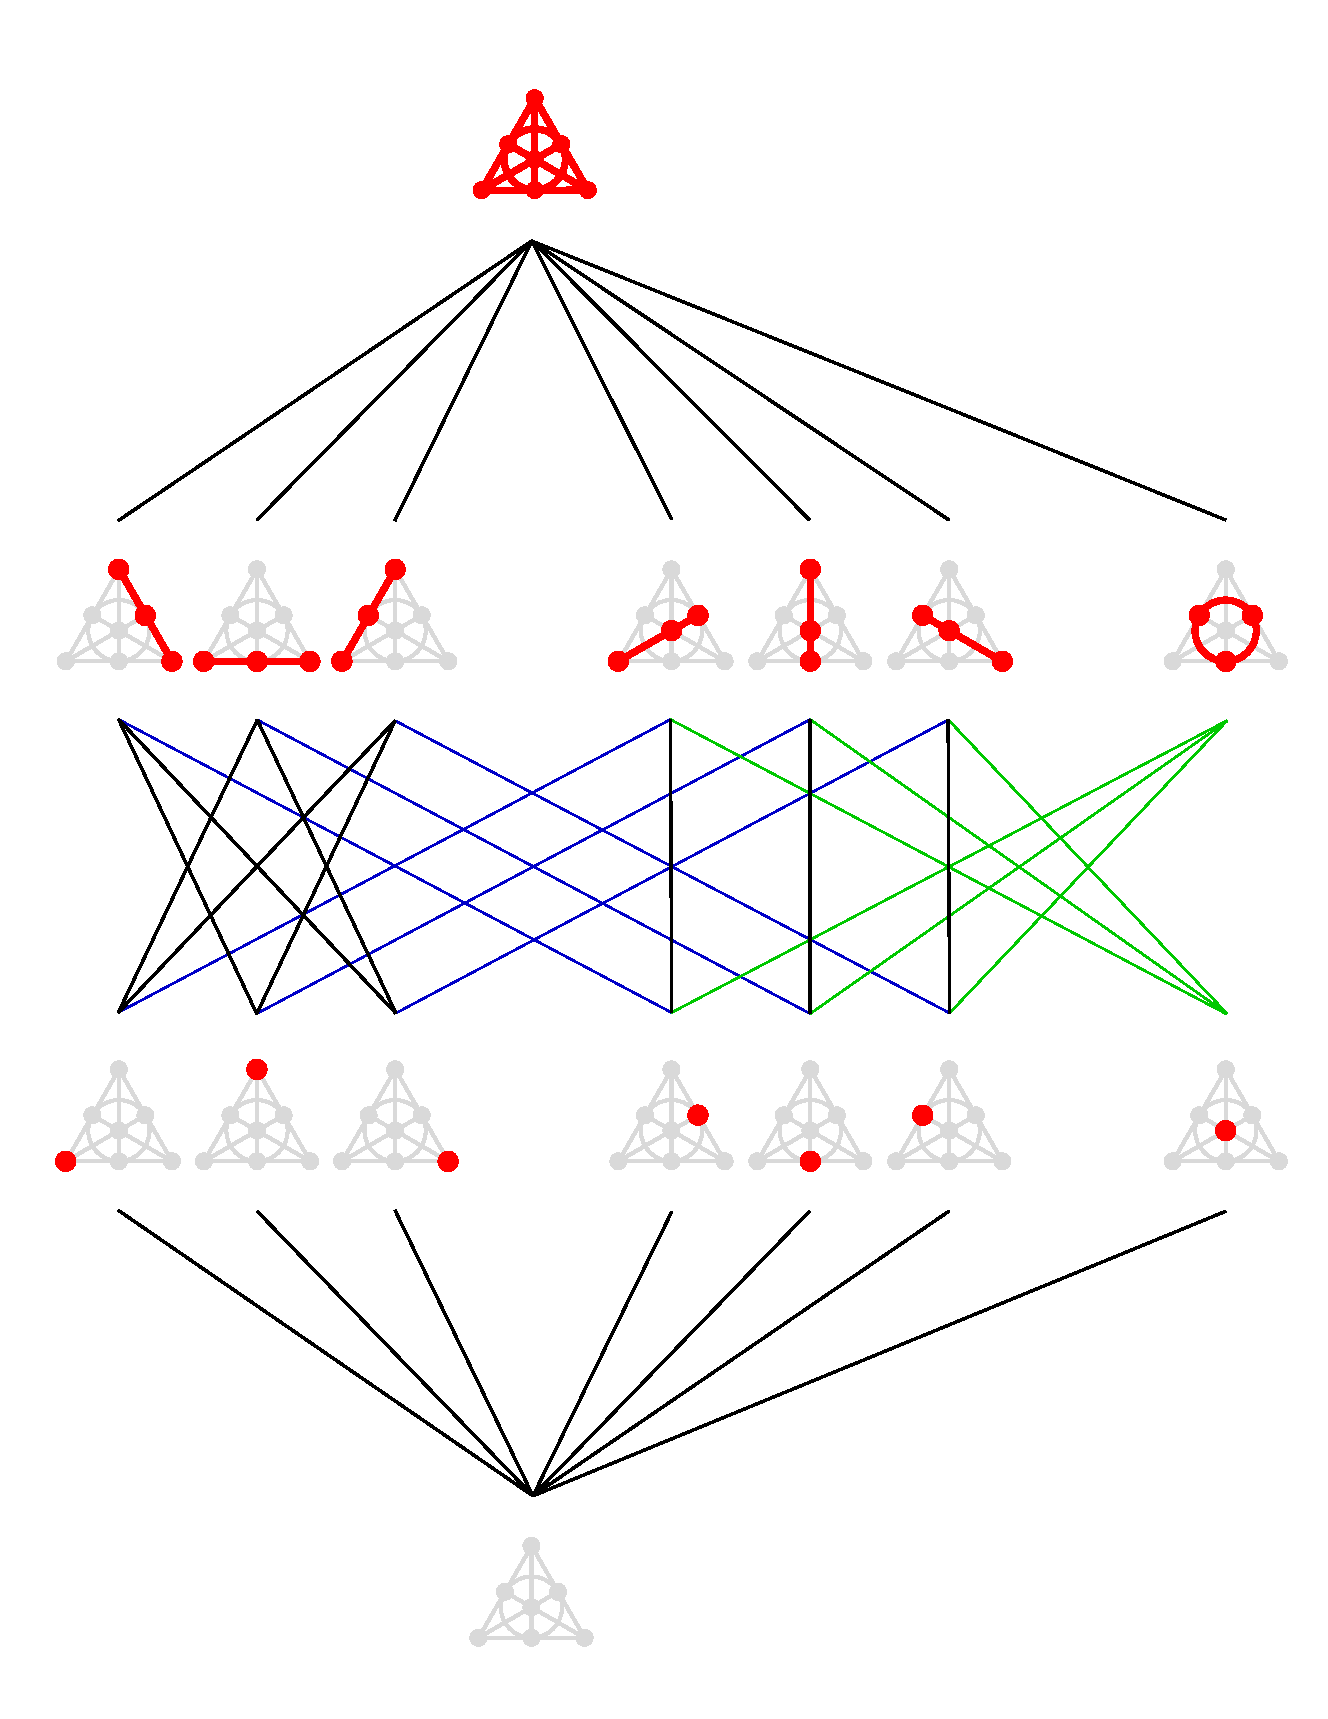
\includegraphics[height=6cm]{Fano_plane_Hasse_diagram} 
    \end{column}
    \begin{column}{0.6\textwidth}%%
      \Emph{Complemented lattice} of types.

      \medskip
      
  \begin{itemize}
  \item \code{SEmpty} and \code{STop}, empty and universal type
  \item \code{SAnd} and \code{SOr}, union and intersection
  \item \code{SNot} complement
  \item \eg, \code{SAnd(Number,SNot(Int)) = Number \& !Int}
  \end{itemize}
      
    \end{column}
  \end{columns}
  
\end{frame}

\newsavebox\adtbox
\begin{lrbox}{\adtbox}
  \begin{minipage}{11cm}
    
\begin{lstlisting}[style=scalaioScala]
abstact class SimpleTypeD {...}
case class SNot(s: SimpleTypeD) extends SimpleTypeD {...}
case class SOr(override val tds: SimpleTypeD*) extends SimpleTypeD {...}
case class SAnd(override val tds: SimpleTypeD*) extends SimpleTypeD {...}
case class SAtomic(ct: Class[_]) extends SimpleTypeD {...}
object SEmpty extends SimpleTypeD {...}
object STop extends SimpleTypeD {...}
case class SSatisfies(f: Any => Boolean, printable:String) extends SimpleTypeD {...}
\end{lstlisting}

  \end{minipage}
\end{lrbox}






\begin{frame}{SimpleTypeD}{Interface to built-in type system}
  
  \begin{itemize}
  \item \code{SAtomic} encapsulates built-in type \code{Class[\_]}\\
    \eg, \code{SAtomic(classOf[Int])}.
  \item \code{SMember} and \code{SEql}, explicit types, encapsulates designated values\\
    \eg, \code{SEql("hello")}, \code{SMember(1,2,3)}
  \item \code{SSatisfies} encapsulates any predicate: \code{Any => Boolean}\\
    \eg, \code{SSatisfies(primep)}.
  \end{itemize}
\end{frame}


\newsavebox\membershipbox
\begin{lrbox}{\membershipbox}
  \begin{minipage}{11cm}
    %% dont re-indent this file
\begin{lstlisting}[style=scalaioScala]
SAtomic(classOf[Int]).typep(-42) // returns true

// returns true
(SAtomic(classOf[String]) || SAtomic(classOf[Int])).typep(7)


// define predicate
def oddp(a:Any):Boolean = {
  a match
    case a:Int => a % 2 != 0
    case _ => false
}

SSatisfies(oddp).typep(36)  // returns false
\end{lstlisting}

  \end{minipage}
\end{lrbox}

\begin{frame}{\code{SimpleTypeD} Membership}
  Type membership question is \Emph{always answerable}.

  \usebox\membershipbox
\end{frame}

\newsavebox\subtypebox
\begin{lrbox}{\subtypebox}
  \begin{minipage}{11cm}
%% dont re-indent this file
\begin{lstlisting}[style=scalaioScala]
val Str:SimpleTypeD = SAtomic(classOf[String])
val Int:SimpleTypeD = SAtomic(classOf[Int])
val Num:SimpleTypeD = SAtomic(classOf[Number])

Str.subtypep(Int)  // returns Some(false)
Int.subtypep(Num)  // returns Some(true)
SSatisfies(oddp).subtypep(Int) // returns None
\end{lstlisting}

  \end{minipage}
\end{lrbox}



\begin{frame}{\code{SimpleTypeD} Subtype}

  Subtype question \Emph{sometimes unanswerable}; \code{subtypep} returns \code{None}

  \usebox\subtypebox

  Unanswerable because:
  \begin{itemize}
  \item Impossible to compute, \eg \code{SSatisfies}.
  \item Code is incomplete.
  \item JVM supports run-time loaded classes.
  \item No dependable way of finding subtypes in JVM $> 8.x$.
  \end{itemize}

\end{frame}
